\chapter{THIẾT KẾ VÀ XÂY DỰNG HỆ THỐNG PYTHON}

\section{Lựa chọn Python và phạm vi xây dựng}

Hệ thống được xây dựng theo hướng Python làm trung tâm. Backend nhận request HTTP, kiểm tra schema, kiểm tra quyền, gọi service nghiệp vụ và thực hiện giao dịch SQL. AI service chỉ là một module được backend gọi khi cần; các chức năng quản lý, lưu dữ liệu và tính KPI vẫn chạy theo quy tắc Python/SQL đã xác định.

Kiến trúc đề xuất dùng FastAPI cho API, Pydantic cho kiểm tra dữ liệu, SQLAlchemy hoặc thư viện truy cập SQLite tương đương cho tầng dữ liệu và một frontend web cho người dùng. Cách tổ chức này chuyển yêu cầu khảo sát và DDL thành hệ thống Python có thể chạy thử.

\section{Kiến trúc hệ thống}

\begin{figure}[h!]
\centering
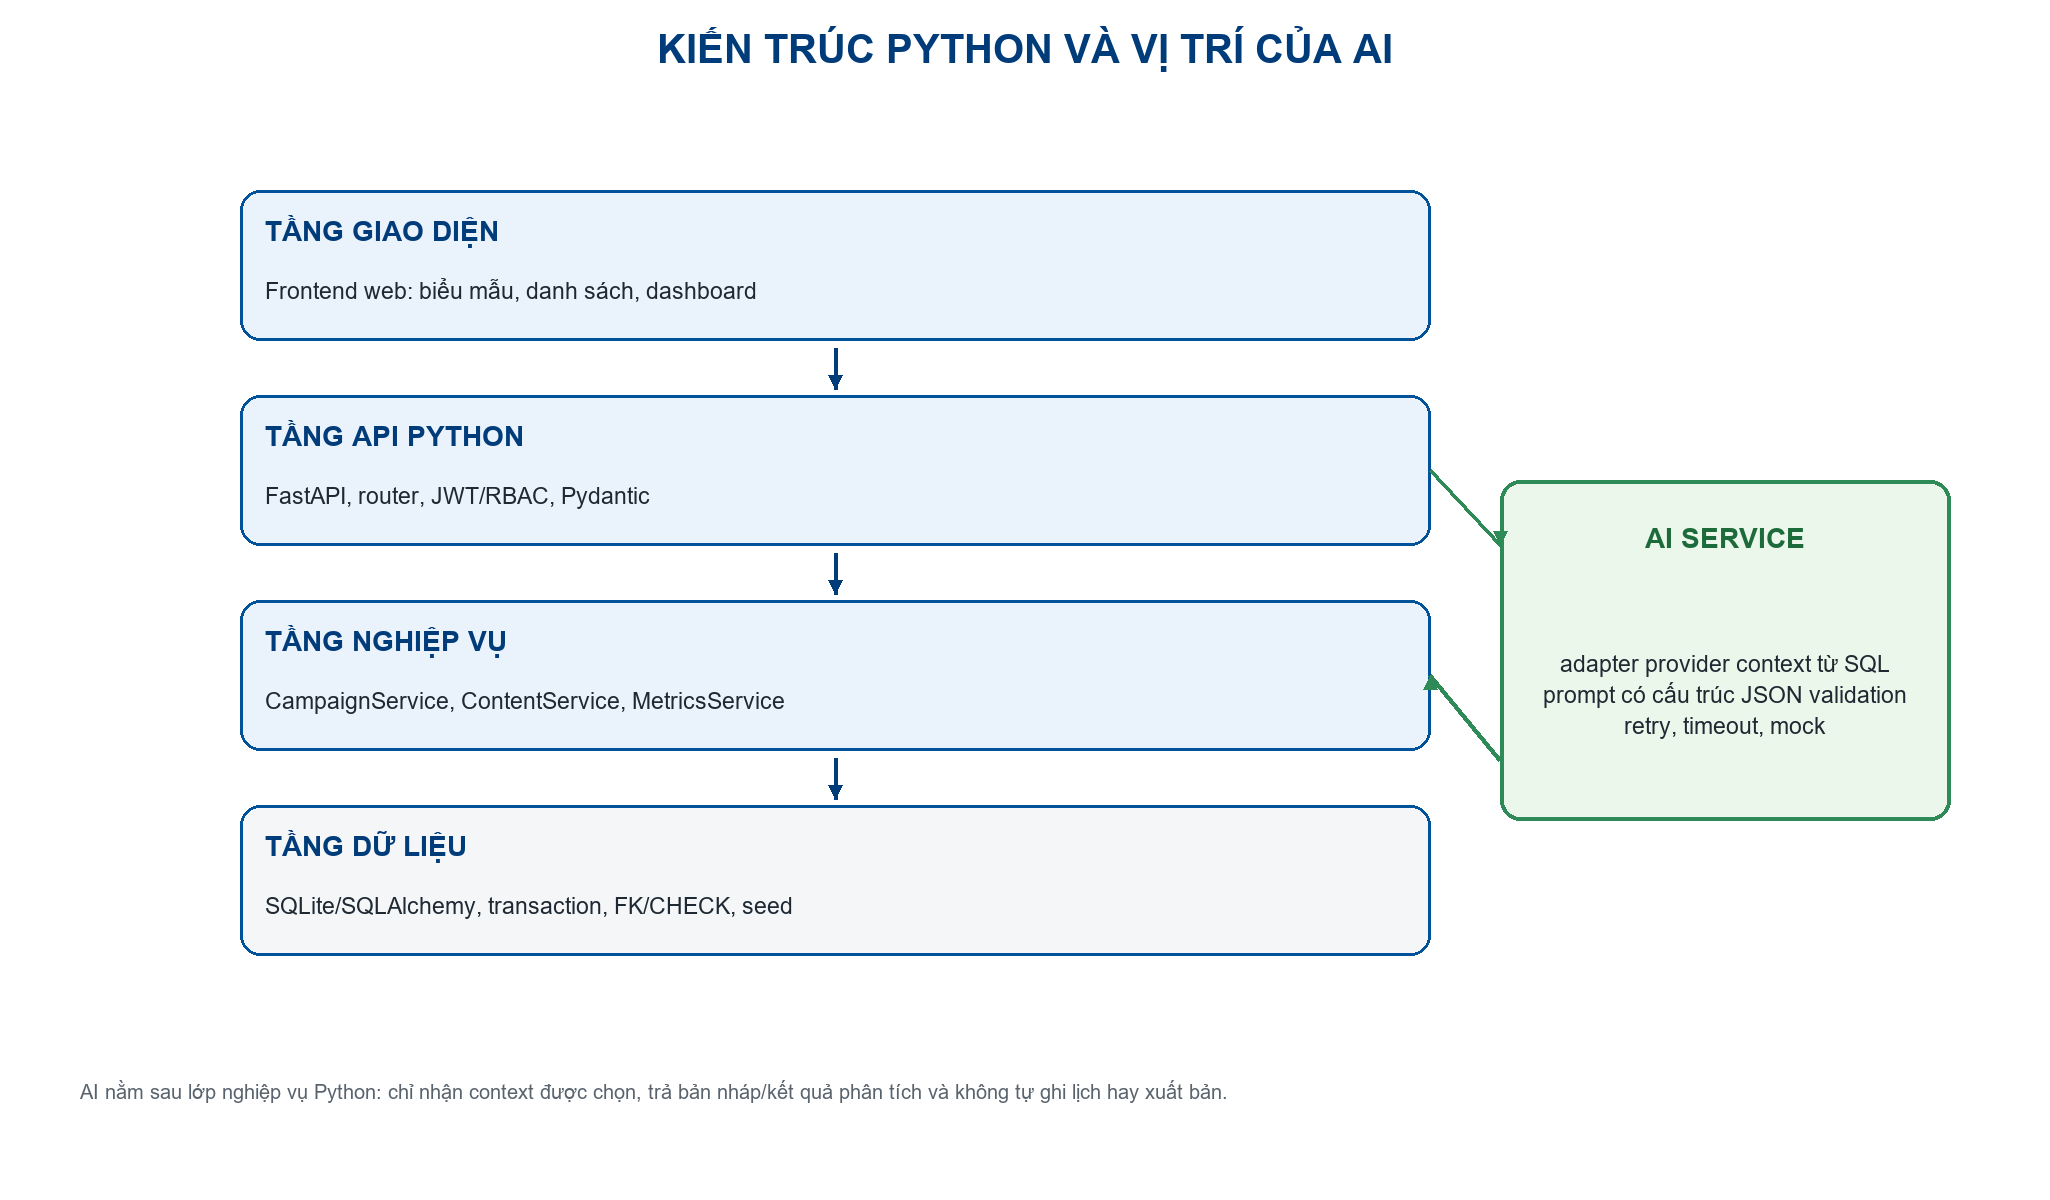
\includegraphics[width=\textwidth]{images/architecture.png}
\caption{Kiến trúc Python và vị trí của AI service}
\end{figure}

\begin{table}[h!]
\centering
\small
\caption{Trách nhiệm của các tầng}
\begin{tabularx}{\textwidth}{|L{3.0cm}|Y|Y|}
\hline
\textbf{Tầng} & \textbf{Thành phần} & \textbf{Trách nhiệm}\\\hline
Giao diện & Form, danh sách, dashboard & Nhận dữ liệu, hiển thị trạng thái và thông báo; không tự quyết định quyền.\\\hline
API Python & FastAPI router, dependency, Pydantic & Nhận request, xác thực, phân quyền và trả mã HTTP rõ ràng.\\\hline
Nghiệp vụ & Service và repository & Kiểm tra quy tắc chiến dịch, trạng thái, CRUD, KPI và giao dịch.\\\hline
Dữ liệu & SQLite/SQLAlchemy, DDL, seed & Lưu bản ghi, thực thi PK/FK/CHECK/UNIQUE và truy vấn báo cáo.\\\hline
AI service & Adapter, prompt, parser, log & Nhận context được phép, gọi AI, kiểm tra output và trả bản nháp/tóm tắt.\\\hline
\end{tabularx}
\end{table}

\section{Cấu trúc thư mục Python}

\begin{lstlisting}[language={},caption={Cấu trúc mã nguồn đề xuất}]
backend/
|-- app/
|   |-- main.py
|   |-- api/              # auth, users, products, campaigns, contents
|   |-- core/             # settings, security, dependencies
|   |-- db/               # engine, session, ddl, seed
|   |-- models/           # SQLAlchemy models
|   |-- schemas/          # Pydantic request/response
|   |-- repositories/     # SQL queries and transactions
|   |-- services/         # campaign, content, metrics, ai service
|   +-- tests/
|-- .env.example
|-- requirements.txt
+-- README.md
\end{lstlisting}

\noindent\textbf{Nguyên tắc:} router không tự nối chuỗi SQL; schema không chứa logic gọi model; service xử lý quy trình; repository nhận tham số đã kiểm tra. DDL và seed được đặt riêng để có thể chạy lại và đối chiếu với ERD.

\section{Đăng nhập và phân quyền RBAC}

Mỗi request được kiểm tra theo chuỗi: đọc Bearer token, giải mã JWT bằng secret từ môi trường, lấy người dùng, kiểm tra trạng thái hoạt động và kiểm tra vai trò. Manager và Marketer dùng chung đăng nhập nhưng có quyền khác nhau ở endpoint. Endpoint duyệt nội dung phải kiểm tra Manager ở backend, không chỉ ẩn nút trên giao diện.

\begin{lstlisting}[language=Python,caption={Dependency kiểm tra JWT và vai trò}]
oauth2_scheme = OAuth2PasswordBearer(tokenUrl="/api/auth/login")

def current_user(token: str = Depends(oauth2_scheme)):
    payload = decode_jwt(token, settings.jwt_secret)
    user = user_repository.find_by_id(payload["sub"])
    if user is None or not user.is_active:
        raise HTTPException(status_code=401, detail="invalid token")
    return user

def require_role(*allowed_roles):
    def checker(user=Depends(current_user)):
        if user.role not in allowed_roles:
            raise HTTPException(status_code=403, detail="forbidden")
        return user
    return checker

@router.post("/contents/{content_id}/approve")
def approve(content_id: int,
            user=Depends(require_role("MANAGER"))):
    return content_service.approve(content_id, user.id)
\end{lstlisting}

\begin{table}[h!]
\centering
\small
\caption{Ý nghĩa các dòng mã Python trong luồng đăng nhập và phân quyền}
\begin{tabularx}{\textwidth}{|L{4.0cm}|Y|}
\hline
\textbf{Dòng hoặc khối mã} & \textbf{Ý nghĩa}\\\hline
\texttt{OAuth2PasswordBearer} & Đọc Bearer token do client gửi trong request.\\\hline
\texttt{decode\_jwt(...)} & Kiểm tra chữ ký và giải mã token để lấy định danh người dùng.\\\hline
\texttt{Depends(current\_user)} & Buộc endpoint xác thực người dùng trước khi chạy nghiệp vụ.\\\hline
\texttt{require\_role(...)} & Chỉ cho các vai trò được khai báo đi qua endpoint.\\\hline
\texttt{@router.post(...)} & Ánh xạ một request HTTP POST vào hàm xử lý tương ứng.\\\hline
\texttt{HTTPException(401/403)} & Trả lỗi rõ ràng khi chưa xác thực hoặc không đủ quyền.\\\hline
\end{tabularx}
\end{table}

\section{CRUD và quy tắc nghiệp vụ}

\subsection{CRUD dữ liệu nền}

Manager có thể tạo nhóm sản phẩm, sản phẩm và kênh. Khi tạo sản phẩm, Python kiểm tra các trường bắt buộc; SQL tiếp tục kiểm tra \texttt{category\_id}, giá, trạng thái và tên trùng. Không cho xóa nhóm khi còn sản phẩm tham chiếu. Các lỗi này phải được trả về thành thông báo có thể sửa.

\begin{lstlisting}[language=Python,caption={Ví dụ endpoint tạo sản phẩm}]
@router.post("/products", status_code=201)
def create_product(payload: ProductCreate,
                   db=Depends(get_db),
                   user=Depends(require_role("MANAGER"))):
    category = product_repository.get_category(db, payload.category_id)
    if category is None:
        raise HTTPException(400, "category does not exist")
    product = product_service.create(db, payload, user.id)
    return ProductResponse.model_validate(product)
\end{lstlisting}

\subsection{CRUD chiến dịch, nội dung và lịch}

Khi tạo chiến dịch, service kiểm tra sản phẩm, người phụ trách, ngày và ngân sách. Nội dung có thể là DRAFT do người viết hoặc AI\_DRAFT do mô-đun AI tạo. Marketer có thể sửa và gửi PENDING. Manager chỉ được duyệt hoặc từ chối nội dung PENDING; nội dung REJECTED phải có lý do. Chỉ APPROVED mới được tạo \texttt{marketing\_schedules}.

\begin{table}[h!]
\centering
\small
\caption{Các bước chuyển trạng thái nghiệp vụ}
\begin{tabularx}{\textwidth}{|C{2.0cm}|C{2.2cm}|Y|Y|}
\hline
\textbf{Trạng thái hiện tại} & \textbf{Trạng thái tiếp theo} & \textbf{Ai thực hiện} & \textbf{Điều kiện}\\\hline
DRAFT & PENDING & Marketer & Đủ tiêu đề, nội dung, chiến dịch và kênh.\\\hline
AI\_DRAFT & PENDING & Marketer & Đã rà soát bản nháp và nguồn context.\\\hline
PENDING & APPROVED & Manager & Nội dung đạt yêu cầu.\\\hline
PENDING & REJECTED & Manager & Có lý do từ chối.\\\hline
APPROVED & PUBLISHED & Quy trình xuất bản & Có lịch hoặc thao tác xuất bản hợp lệ.\\\hline
APPROVED & PLANNED & Người có quyền & Tạo lịch với thời điểm hợp lệ.\\\hline
\end{tabularx}
\end{table}

\section{Tìm kiếm, lọc, phân trang và báo cáo}

Danh sách chiến dịch được lọc theo trạng thái và khoảng ngày; nội dung được tìm theo tiêu đề, kênh hoặc trạng thái; chỉ số được lọc theo chiến dịch, kênh và ngày. Mọi tham số được truyền vào query parameter và bind vào câu lệnh SQL/ORM. \texttt{limit} và \texttt{offset} có giá trị mặc định để tránh trả về quá nhiều bản ghi.

\begin{table}[h!]
\centering
\small
\caption{Tham số truy vấn của các màn hình}
\begin{tabularx}{\textwidth}{|L{3.0cm}|Y|Y|}
\hline
\textbf{Màn hình} & \textbf{Bộ lọc} & \textbf{Kết quả}\\\hline
Chiến dịch & status, start\_from, end\_to, owner\_id, limit, offset & Danh sách chiến dịch và tổng số bản ghi.\\\hline
Nội dung & keyword, status, channel\_id, campaign\_id, limit, offset & Nội dung phù hợp và trạng thái duyệt.\\\hline
Dashboard & campaign\_id, channel\_id, date\_from, date\_to & Views, Clicks, Conversions, Cost, Revenue và KPI.\\\hline
\end{tabularx}
\end{table}

\subsection{Công thức KPI trong service Python}

\begin{align}
CTR &= \frac{Clicks}{Views}\times 100\% \\
CPC &= \frac{Cost}{Clicks} \\
CPA &= \frac{Cost}{Conversions} \\
ROI &= \frac{Revenue-Cost}{Cost}\times 100\%
\end{align}

Khi mẫu số bằng 0, service trả \texttt{None} hoặc \texttt{N/A} theo quy ước giao diện và ghi rõ lý do. Công thức không giao cho AI; SQL/Python là nơi tính kết quả để bảo đảm lặp lại được.

\section{Giao diện và phản hồi trạng thái}

\begin{table}[h!]
\centering
\small
\caption{Màn hình chính và thao tác của người dùng}
\begin{tabularx}{\textwidth}{|L{3.1cm}|Y|Y|}
\hline
\textbf{Màn hình} & \textbf{Marketer} & \textbf{Manager}\\\hline
Đăng nhập & Đăng nhập và xem phiên & Đăng nhập và xem phiên\\\hline
Sản phẩm & Xem & Thêm, sửa, xóa và kiểm tra nhóm\\\hline
Chiến dịch & Xem chiến dịch được phân công & Tạo, sửa, điều chỉnh ngân sách và phân công\\\hline
Nội dung & Tạo, sửa, gọi AI, gửi duyệt & Xem, duyệt hoặc từ chối có lý do\\\hline
Lịch đăng & Tạo theo quyền và theo dõi & Tạo, hủy và theo dõi\\\hline
Báo cáo & Nhập số liệu, xem KPI & Xem KPI, lọc và đánh giá\\\hline
\end{tabularx}
\end{table}

Thông báo cần nói rõ thao tác tiếp theo, ví dụ: Thiếu tên sản phẩm; bạn không có quyền duyệt; nội dung chưa được APPROVED nên chưa thể lập lịch. Trạng thái phải có cả nhãn chữ và màu phụ trợ. Bản nháp người dùng đang sửa phải được giữ lại khi API hoặc AI gặp lỗi.

\section{Xử lý lỗi và cấu hình}

\begin{table}[h!]
\centering
\small
\caption{Mã lỗi và cách phản hồi}
\begin{tabularx}{\textwidth}{|L{3.2cm}|C{1.5cm}|Y|}
\hline
\textbf{Tình huống} & \textbf{Mã} & \textbf{Phản hồi}\\\hline
Thiếu trường hoặc sai kiểu & 422 & Nêu tên trường và giá trị cần sửa.\\\hline
Chưa đăng nhập hoặc token hết hạn & 401 & Yêu cầu đăng nhập lại.\\\hline
Sai vai trò & 403 & Thông báo tài khoản không có quyền thao tác.\\\hline
Không tìm thấy dữ liệu & 404 & Nêu tài nguyên không tồn tại.\\\hline
Vi phạm FK, UNIQUE hoặc CHECK & 400 & Giải thích quy tắc dữ liệu bị vi phạm.\\\hline
Lỗi kết nối hoặc server & 500/503 & Giữ dữ liệu đang sửa và ghi mã truy vết.\\\hline
\end{tabularx}
\end{table}

Chuỗi kết nối CSDL, JWT secret và API key được đọc từ biến môi trường. Tệp \texttt{.env.example} chỉ chứa tên biến và giá trị thay thế. Khi thiếu secret bắt buộc, ứng dụng phải dừng với lỗi cấu hình rõ ràng. README cần ghi thứ tự tạo môi trường Python, cài dependency, sao chép env, chạy DDL, seed dữ liệu, khởi động server và chạy test.

\section{Bộ 20 ca kiểm thử của toàn hệ thống}

Các ca dưới đây phủ các yêu cầu P01--P26 theo nhóm. Đây là mẫu kế hoạch nghiệm thu; cột trạng thái phải được điền từ lần chạy thật, kèm ảnh hoặc log có ngày chạy, phiên bản mã nguồn và người xác nhận.

\begingroup
\scriptsize
\setlength{\LTleft}{0pt}
\setlength{\LTright}{0pt}
\begin{longtable}{|C{0.9cm}|L{4.5cm}|L{5.3cm}|C{1.5cm}|}
\caption{Bộ 20 ca kiểm thử từ quản lý đến AI}\label{tab:test20-v4}\\
\hline
\textbf{Mã} & \textbf{Kịch bản} & \textbf{Kỳ vọng} & \textbf{Trạng thái kiểm chứng}\\
\hline\endfirsthead
\hline
\textbf{Mã} & \textbf{Kịch bản} & \textbf{Kỳ vọng} & \textbf{Trạng thái kiểm chứng}\\
\hline\endhead
\texttt{TC01} & Đăng nhập đúng tài khoản & Nhận token và vào dashboard & Chưa chạy\\\hline
\texttt{TC02} & Sai mật khẩu & Trả 401, không lộ chi tiết & Chưa chạy\\\hline
\texttt{TC03} & Token hết hạn & Trả 401 và yêu cầu đăng nhập lại & Chưa chạy\\\hline
\texttt{TC04} & Marketer gọi endpoint duyệt & Trả 403 và không đổi trạng thái & Chưa chạy\\\hline
\texttt{TC05} & Tạo nhóm sản phẩm đủ trường & Lưu bản ghi, tên không trùng & Chưa chạy\\\hline
\texttt{TC06} & Tạo sản phẩm với nhóm sai & Trả lỗi FK, không lưu & Chưa chạy\\\hline
\texttt{TC07} & Nhập giá âm & Trả lỗi CHECK, không lưu & Chưa chạy\\\hline
\texttt{TC08} & Sửa và xóa sản phẩm & Cập nhật đúng; chặn xóa khi còn tham chiếu & Chưa chạy\\\hline
\texttt{TC09} & Tạo chiến dịch ngày ngược & Trả lỗi, không tạo chiến dịch & Chưa chạy\\\hline
\texttt{TC10} & Lọc chiến dịch theo trạng thái & Chỉ trả bản ghi đúng bộ lọc & Chưa chạy\\\hline
\texttt{TC11} & Tìm kiếm nội dung theo từ khóa & Trả danh sách phù hợp có phân trang & Chưa chạy\\\hline
\texttt{TC12} & Sắp xếp báo cáo theo doanh thu & Thứ tự tăng/giảm đúng yêu cầu & Chưa chạy\\\hline
\texttt{TC13} & Tính KPI khi Views bằng 0 & Không chia cho 0; trả N/A & Chưa chạy\\\hline
\texttt{TC14} & Tính ROI khi Cost bằng 0 & Không chia cho 0; cảnh báo cấu hình & Chưa chạy\\\hline
\texttt{TC15} & Tạo nội dung thủ công & Lưu DRAFT và người tạo & Chưa chạy\\\hline
\texttt{TC16} & Gửi nội dung để duyệt & DRAFT/AI\_DRAFT chuyển PENDING & Chưa chạy\\\hline
\texttt{TC17} & Manager từ chối thiếu lý do & Không chuyển trạng thái; yêu cầu lý do & Chưa chạy\\\hline
\texttt{TC18} & Chỉ lập lịch nội dung APPROVED & Nội dung chưa duyệt bị từ chối & Chưa chạy\\\hline
\texttt{TC19} & AI trả JSON sai hoặc timeout & Giữ bản nháp cũ, trả lỗi có thể thử lại & Chưa chạy\\\hline
\texttt{TC20} & AI trả kết quả hợp lệ & Lưu AI\_DRAFT, source\_ids và hiển thị để người duyệt & Chưa chạy\\\hline
\end{longtable}
\endgroup

\section{Minh chứng cần nộp khi hoàn thiện hệ thống}

\begin{enumerate}
  \item Cây thư mục Python, file \texttt{requirements.txt}, \texttt{README.md} và \texttt{.env.example}.
  \item Lệnh SQL tạo bảng, ảnh ERD được đối chiếu với DDL và dữ liệu seed.
  \item Ảnh hoặc log đăng nhập, RBAC, CRUD, tìm kiếm, dashboard và các mã lỗi.
  \item Log 20 ca kiểm thử có phiên bản mã nguồn và ngày chạy.
  \item Ảnh màn hình bản nháp, duyệt nội dung và trạng thái lịch đăng.
\end{enumerate}

\section{Kết luận chương}

Các yêu cầu khảo sát đã được chuyển thành module Python, bảng SQL, service và kế hoạch kiểm thử. Mô hình này giúp người chấm theo dõi từ yêu cầu đến hệ thống; phần AI ở chương sau chỉ được gọi sau khi luồng Python, CSDL và quyền đã rõ.
